% Metódy inžinierskej práce
 \documentclass[10pt,twoside,slovak,a4paper]{article}
\usepackage[slovak]{babel}
%\usepackage[T1]{fontenc}
\usepackage[IL2]{fontenc} % lepšia sadzba písmena Ľ než v T1
\usepackage[utf8]{inputenc}
\usepackage{graphicx}
\usepackage{url} % príkaz \url na formátovanie URL
\usepackage{hyperref} % odkazy v texte budú aktívne (pri niektorých triedach dokumentov spôsobuje posun textu)
\usepackage{cite}
\usepackage{wrapfig}
\usepackage{amsmath}

\pagestyle{headings}

\title{text-to-image search/ image-to-image search\thanks{Semestrálny projekt v predmete Metódy inžinierskej práce, ak. rok 2023/24, vedenie:Vladimír Mlynarovič}} 

\author{Ondrej Krajčovič\\[2pt]
	{\small Slovenská technická univerzita v Bratislave}\\
	{\small Fakulta informatiky a informačných technológií}\\
	{\small \texttt{xkrajcovico@stuba.sk}}
	}
\date{\small 5.november 2023}






\begin{document}

\maketitle

\begin{abstract}
Článok poskytuje stručný opis fungovania, využitia a možností spätného vyhľadávania obrázkov (eng.: reverse image search, alebo image-pto-image-search)
a vyhľadávania obrázkov pomocou textu (eng.: text-to-image search).
Nakoľko ľudia prirodzene vyjadrujú svoje myšlienky slovami, je pre nás pomerne ťažké komunikovať pomocou obrázkov, obzvlášť ich vyhľadávanie je občas pomerne neefektívne. 
Komunikácia sa však v posledných rokoch veľmi zmenila nástupom moderných, technologicky vyspelých komunikačných kanálov(eng.: Mass media). Vyjadrovanie myšlienok graficky sa teda zdá byť na dosah ruky, problémom je však vyhľadanie daných grafík v databázach a na internete. Článok rozoberá nedávny pokrok, ťažkosti a nové nápady, ktoré spájajú rôzne typy informácií, predovšetkým vizuálne a modálne, a ukazuje, aké dôležité sú tieto oblasti v dnešnej digitálnej dobe.

\end{abstract}
\newpage






\section{Úvod - Ľudské vnemy a sémantika} \label{01}
Ľudský mozog vníma informácie pomocou zmyslov. Dominantný zmysel u človeka je zrak, je nám preto iba prirodzené vnímať informácie pomocou obrázkov. Ľudská schopnosť sémanticky pochopiť obraz je dokonca oveľa rýchlejšia ako schopnosť vnímať text. Toto je presne dôvod, prečo sú dôležité informácie často znázorňované pomocou rôznych grafík, piktogramov~\ref{piktogram}. Rôzne abecedy sa dokonca vyvíjali priamo z grafických znázornení objektov ktoré sa vyskytovali v okolí osôb vyvíjajúcich dané písmo.
Pre počítače však vizuálny spôsob vnímania komplexných informácií nie je prirodzený. Ako teda vnímajú stroje informáciu? 
\begin{figure*}[htb!]\label{piktogram}
  \centering
  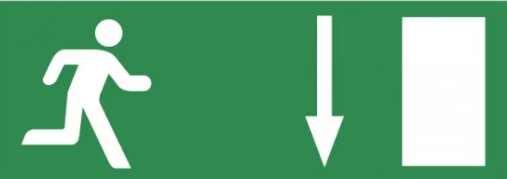
\includegraphics[width=0.48\textwidth]{images/piktogram.png} 
  \caption{ukážka piktogramu}
\end{figure*}


\section{funkcia metadát (metaúdajov) pri hľadaní obrázkov} \label{02}
Metadáta sú všeobecne informácie, respektíve dáta, ktoré nemusia byť priamo súčasťou daného súboru, ale ich primárnou funkciou je opísať, čo sa v danom súbore nachádza. V našom prípade sú to teda informácie slovne opisujúce čo sa na obrázku nachádza, kde a kedy bol obrázok vytvorený (tieto informácie platia predovšetkým o fotografiách)~\ref{metadata}. Tento kontext teda odstraňuje rozdiel medzi jazykovým a vizuálnym obsahom a umožňuje získať presnejšie a relevantnejšie výsledky vyhľadávania. Slúžia teda ako kľúč ku spracovaniu vizuálnych informácií, napríklad pomocou queries, čo znamená, že vyhľadávací algoritmus vyhľadáva na základe nie iba grafických, ale predovšetkým textových informácií. Takéto vyhľadávanie sa nazýva text to image search.
\begin{figure*}\label{metadata}
  \centering
  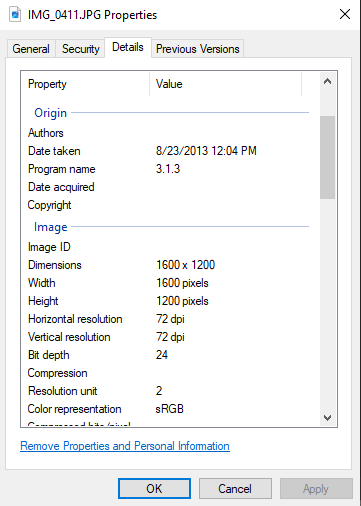
\includegraphics[width=0.48\textwidth]{images/metadata.png} 
  \caption{ukážka zobrazenia metadát na konkrétnom obrázku v prostredí windows}
\end{figure*}


\section{Text-to-image search} \label{03}
Queries,  textový vstup poskytnutým používateľmi sa pri tomto procese porovnáva z potencionálne zhodnými informáciami zapísanými vo forme metadát k prislúchajúcim obrázkom. V prípade že do vyhľadávača na internete zadáme vstup: “golden bridge“, pomocou metadát vyhľadá súvisiace obrázky, ktorých metadáta obsahujú text: “ golden bridge“~\ref{metadata_google}
\begin{figure*}[htb!]\label{metadata_google}
  \centering
  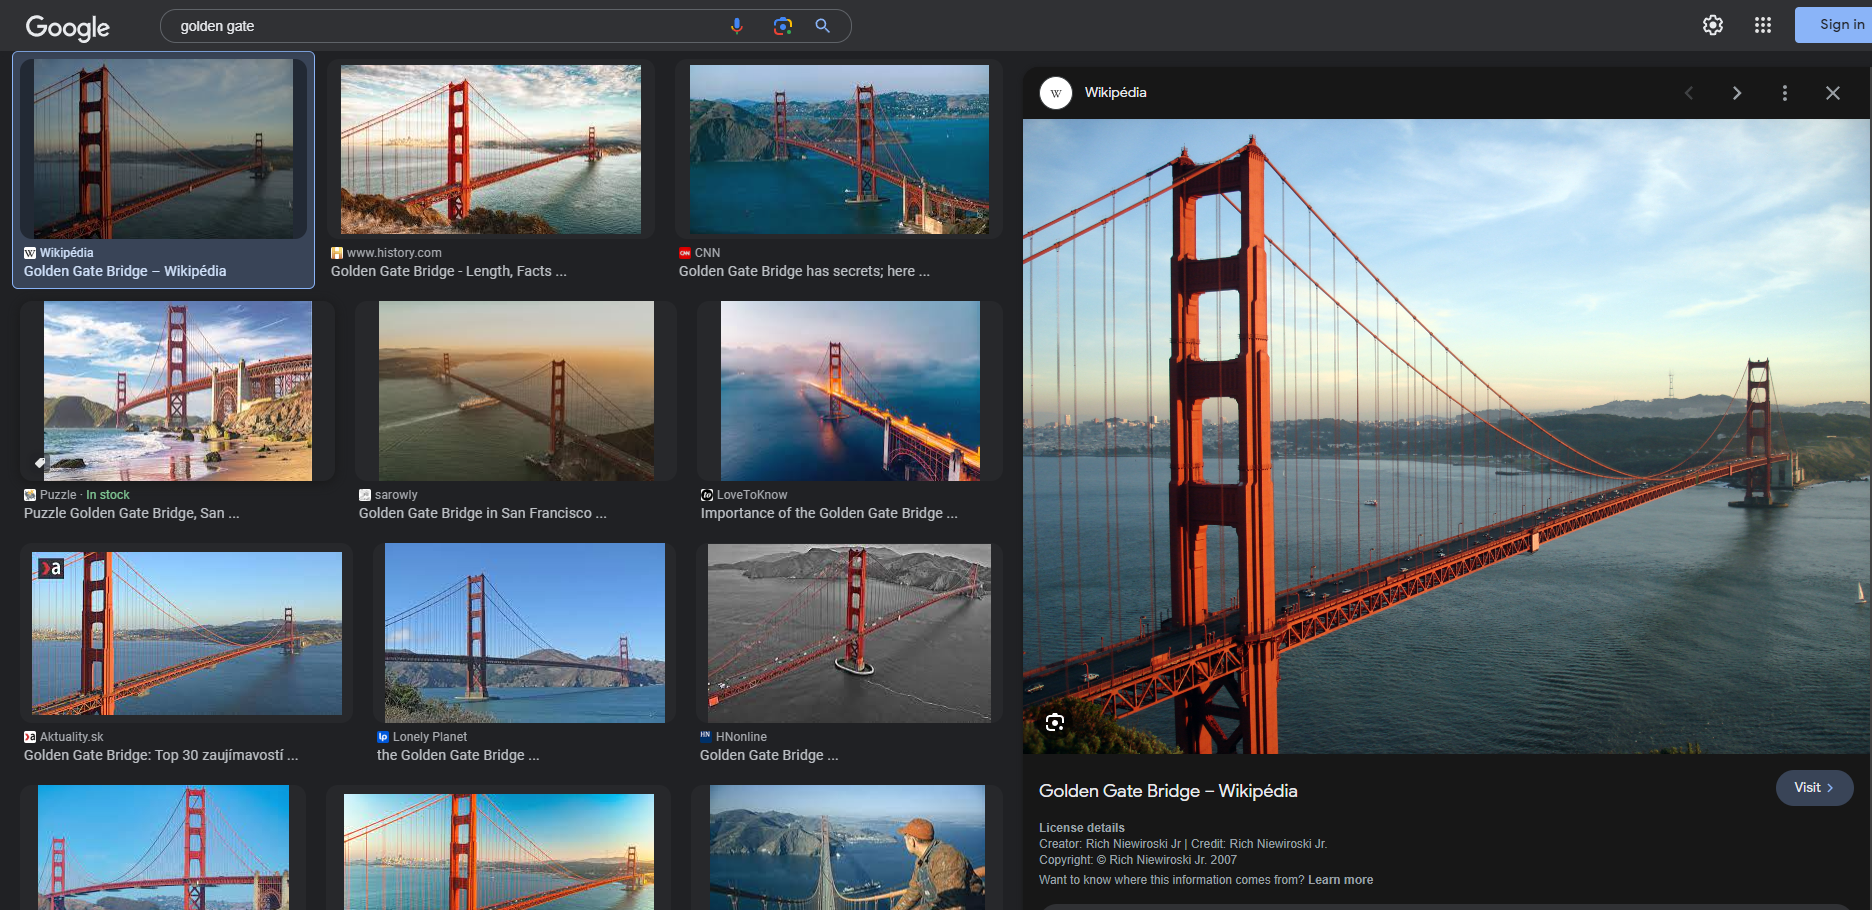
\includegraphics[width=0.48\textwidth]{images/metadata_google.png} 
  \caption{ukážka využitia metadát pri hľadaní na internete}
\end{figure*}


\newpage




\section{Neefektívnosť pri vyhľadávaní obrázkov} \label{04}
V prípade, že však pri vyhľadávaní chceme hľadať pomocou vizuálneho vstupu, a nie pomocou textových queries, musíme postupovať inak. Jednou z možností je preložiť grafickú informáciu, ktorú nám poskytuje vstupný obrázok do textovej podoby, a následne pomocou text-to-image vyhľadáva. Tento proces je však pomerne neefektívny, a jeho výsledky mnohokrát nezodpovedajú našim očakávaniam natoľko aby sme s nimi boli spokojní.
Optimálnym riešením tohto problému by teda bol počítač, schopný vnímať a pracovať s informáciami priamo na úrovni grafického rozpätia týchto informácií.

\newpage


\section{image-to-image search} \label{05}
Je to vyhľadávanie obrázkov kedy je vstupom(query) iný obrázok. Umožňuje používateľom nájsť obrázky podobné danému vyhľadávaciemu obrázku, často analyzovaním vizuálnych prvkov, ako sú farba, tvar a textúra

\section{Reverse Image Search} \label{08}
Algoritmus používaný na image-to-image search. pracuje v nasledovných krokoch: najprv vyhľadáva špecifické črty obrázka, ďalej porovnáva jednotlivé črty s črtami iných obrázkov v databáze (napríklad na internete). Nakoniec vyhodnotí najpodobnejšie obrázky a vráti ich používateľovi. počas tohto procesu nemusí algoritmus používať iba črty daného obrázka, môže si pomáhať aj metadátami

\section{Sémantika} \label{09}
Vedci boli schopní graficky zobraziť~\cite{Deep_image_reconstruction_from_human_brain_activity } neurónové signály v ľudskom mozgu priamo pri procese spracovávania vizuálnych podnetov ~\ref{brain}, a následne aj počas toho ako si daný človek spomínal na daný vizuálny podnet. Výsledkom nebol jasný obraz, zhodný s vizuálnym podnetom, ktorý bol človeku poskytnutý, ale pomerne rozmazaná a skreslená informácia. Mňa osobne zaujala podobnosť tejto grafiky s obrázkami ktoré generovala umelá inteligencia. 
\begin{figure*}[htb!]\label{brain}
  \centering
  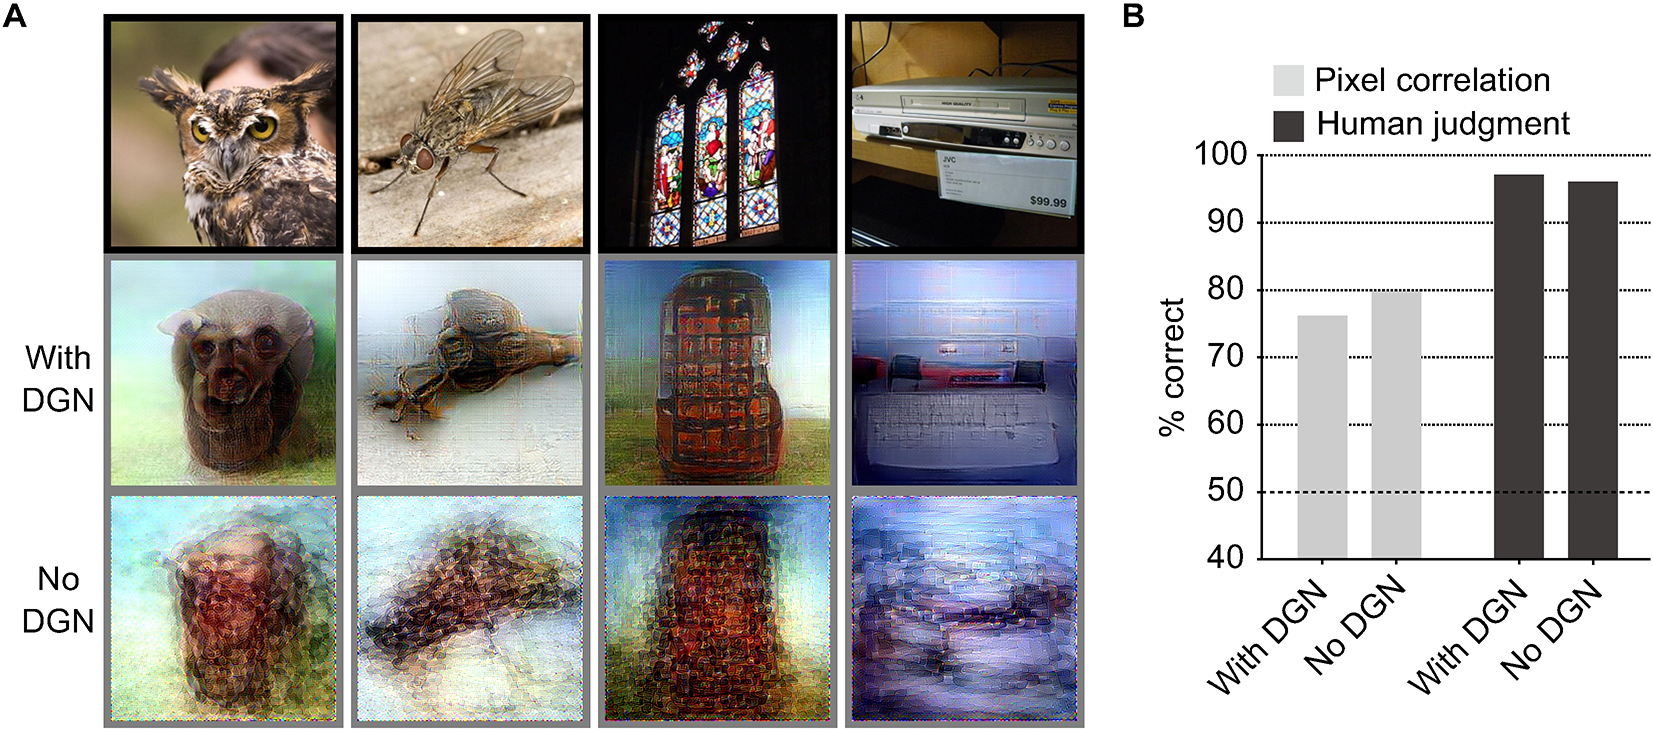
\includegraphics[width=0.48\textwidth]{images/brain_image.png} 
  \caption{Vizuálne zobrazenie signálov z ľudského mozgu pri spracovávaní obrázkov}
\end{figure*}
\begin{figure*}[htb!]\label{AI_prompt}
  \centering
  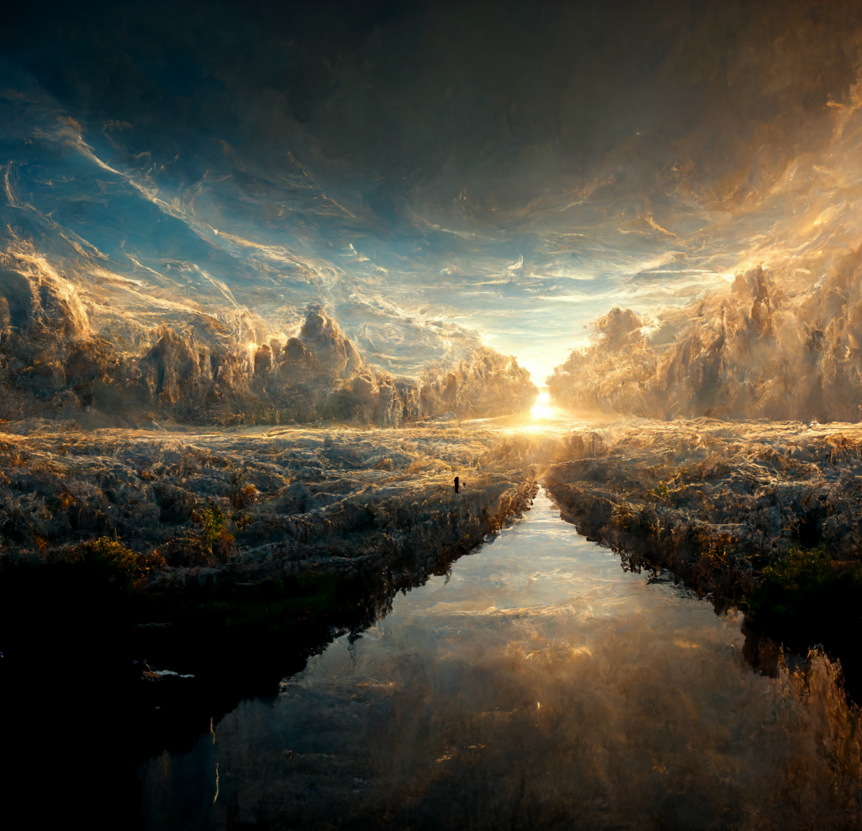
\includegraphics[width=0.48\textwidth]{images/AI_prompt.png} 
  \caption{Obrázok generovaný pomocou umelej inteligencie}
\end{figure*}


\section{AI a deep learning} \label{10}

Spoločnosť OpenAI publikovala v roku 2021 nástroj s názvom CLIP(Contrastive Language-Image Pre-Training~\ref{clip}), Je to pomerne efektívna umelá inteligencia~\ref{clip_efektivita} nástroj, ktorý môže generovať textové opisy obrázkov, hľadať obrázky založené na textových queries a vykonávať rôzne úlohy, ktoré si vyžadujú hlboké pochopenie obrazov aj textu
\begin{figure*}[htb!]\label{clip}
  \centering
  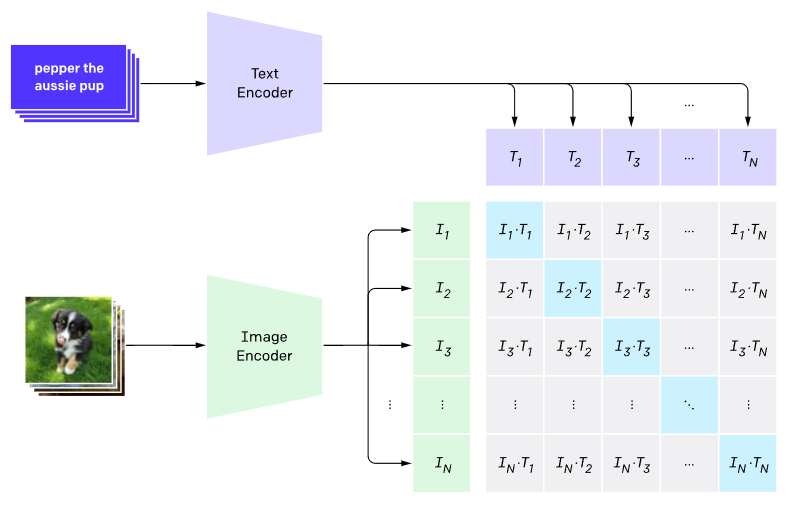
\includegraphics[width=0.48\textwidth]{images/image_encoding.png} 
  \caption{CLIP spracováva vizuálne informácie a metadáta pri trénovaní}
\end{figure*}
\begin{figure*}[htb!]\label{clip_efektivita}
  \centering
  \includegraphics[width=0.48\textwidth]{images/CLIP.png} 
  \caption{efektivita nástroja CLIP}
\end{figure*}

\section{Záver} \label{zaver} % prípadne iný variant názvu
Článok sa dotýka tém vyhľadávania, s hlavným zameraním "text-to-image search" a "image-to-image search". Je v ňom vysvetlená dôležitosť a funkcionalita metadát pri vyhľadávaní. Koncept image-to-image search vyhľadávania je čitateľovi taktiež priblížený. Na záver sa článok dotýka témy umelej inteligencie a jej konkrétneho využitia v tejto oblasti

\newpage
\bibliography{literatura}
\bibliographystyle{plain}
\end{document}